\documentclass[11.5pt]{article}

\usepackage{amssymb, amsmath, amsthm, amsfonts, eurosym, geometry, ulem, graphicx, caption, color, setspace, footmisc, pdflscape, array, todonotes, subfig, adjustbox, booktabs, pdfpages, siunitx, setspace, multirow, tikz, appendix}

\usepackage[flushleft]{threeparttable}
%\usepackage{hyperref}
\usepackage{natbib}
\bibliographystyle{econometrica}
%\usepackage[round]{natbib}
\usepackage[applemac]{inputenc}
\usepackage{hyperref}
%\usepackage{xcolor}
%\hypersetup{
%  colorlinks   = true, %Colours links instead of ugly boxes
%  urlcolor     = red, %Colour for external hyperlinks
%  linkcolor    = blue, %Colour of internal links
%  citecolor   = blue %Colour of citations
%}

\geometry{left=1in,right=1in,top=1in,bottom=1in}

\captionsetup{justification=justified}

\setlength{\textwidth}{6in}
\setlength{\oddsidemargin}{.22in}
\setlength{\textheight}{9in}
\setlength{\topmargin}{-0.10in}
\setlength{\headheight}{0.02in}

\normalem

\onehalfspacing
\newtheorem{theorem}{Theorem}
\newtheorem{corollary}[theorem]{Corollary}
\newtheorem{proposition}{Proposition}

\newtheorem{conjecture}{Conjecture}
\newtheorem{example}{Example}
\newtheorem{definition}{Definition}
\newtheorem{assumption}{Assumption}
\newtheorem{remark}{Remark}

%\newenvironment{proof}[1][Proof]{\noindent\textbf{#1.} }{\ \rule{0.5em}{0.5em}}

\newtheorem{hyp}{Hypothesis}
\newtheorem{subhyp}{Hypothesis}[hyp]
\renewcommand{\thesubhyp}{\thehyp\alph{subhyp}}

\newcommand{\red}[1]{{\color{red} #1}}
\newcommand{\blue}[1]{{\color{blue} #1}}

\newcolumntype{L}[1]{>{\raggedright\let\newline\\arraybackslash\hspace{0pt}}m{#1}}
\newcolumntype{C}[1]{>{\centering\let\newline\\arraybackslash\hspace{0pt}}m{#1}}
\newcolumntype{R}[1]{>{\raggedleft\let\newline\\arraybackslash\hspace{0pt}}m{#1}}

\geometry{left=1.0in,right=1.0in,top=1.0in,bottom=1.0in}

\captionsetup{justification=justified}
\renewcommand{\baselinestretch}{1.3}
\newcounter{marginparcounter}
\newcommand{\patopar}[1]{\stepcounter{marginparcounter}$^{(\roman{marginparcounter})}$\marginpar{\color{red}\renewcommand{\baselinestretch}{0.8}\scriptsize$^{(\roman{marginparcounter})}$ PD: #1}}
\renewcommand{\baselinestretch}{1.3}
\setlength{\textwidth}{6in}
\setlength{\oddsidemargin}{.22in}
\setlength{\textheight}{9in}
\setlength{\topmargin}{-0.10in}
\setlength{\headheight}{0.02in}
%\setlength{\parskip}{0.4cm}

\renewcommand{\thesection}{\Roman{section}}
\renewcommand{\thesubsection}{\Alph{subsection}}

\newcommand{\appendixpagenumbering}{
  \break
  \pagenumbering{arabic}
  \renewcommand{\thepage}{\thesection-\arabic{page}}
}



\begin{document}
\title{\Large \textbf{Shocking Business Aspirations: \\
Experimental Evidence from Small-scale Entrepreneurs in a Developing Economy}\thanks {\scriptsize We thank the Abdul Latif Jameel Poverty Action Lab (J-PAL) for hosting our study, in particular Raisa Annisa, Ni Luh Putu Satyaning Pradnya Paramita, Lukman Edwindra, and Dwitri Amalia for excellent research assistance. This paper was produced under the framework of the \textquotedblleft Enabling Innovation and Productivity Growth in Low Income Countries (EIP-LIC/PO5639)" project, funded by the Department for International Development (DFID) of the United Kingdom and implemented by Tilburg University. Additional funding was received by The World Bank and Tilburg Economics Department. Research on the ground was conducted in cooperation with J-PAL South-East Asia and SurveyMETER.}}

\author{Patricio S. Dalton\thanks{\scriptsize Tilburg University, Department of Economics and CentER, Warandelaan 2, 5037 AB, Tilburg, The Netherlands. E-mail corresponding author: \texttt{p.s.dalton@uvt.nl} (corresponding author), \texttt{j.ruschenpohler@uvt.nl}}
\and Julius R\"uschenp\"ohler\footnotemark[2]
\and Bilal Zia\thanks{\scriptsize The World Bank, Development Research Group, 1818 H St. N.W. Washington, D.C. 20433. E-mail: \texttt{bzia@worldbank.org}.}}


\date{\today}
\maketitle
\singlespace

\begin{abstract}
\noindent {Are the growth aspirations of small-scale entrepreneurs responsive to shocks? If so, does initial distance from the efficient frontier determine the direction of change? In a randomized controlled trial in Indonesia, we study an informational shock to entrepreneurial aspirations by distributing a handbook of key business practices implemented by successful local peers. The handbook is complemented with two psychological and implementation nudges: a movie with business role models from the local area who demonstrate their path to success; and personalized business assistance to help entrepreneurs with individual implementation challenges. In line with the theoretical literature, we find that initial distance to the frontier matters. Entrepreneurs with high business aspirations at baseline respond positively to the treatments and increase business aspirations, sales, and profits; while those with low initial aspirations respond negatively and decrease their business aspirations and performance. We find similar heterogeneity in complementary aspirations for children's education and satisfaction with household finances. These results confirm that initial levels of aspirations are crucial in determining how entrepreneurs respond to exogenous aspirational shocks. }\\



\noindent\textbf{Keywords:} Aspirations, Aspirations Failure, Aspirations Frustration, Small-business Growth, Business Performance, Subjective Well-Being, Randomized Control Trial.\\
\noindent\textbf{JEL Codes:};
\end{abstract}
\vfill

\thispagestyle{empty}

\pagebreak

\doublespacing

\setcounter{page}{1}


\section{\textbf{Introduction}}

It is a long-standing puzzle in development economics why poor individuals and small-scale businesses often do not exploit productive investment opportunities \citep[see,][]{Banerjee2014, deMel2008, McKenzie2008, Karlan2010}. Beyond classical work on imperfections in the markets for credit and insurance \citep[e.g.,][]{Banerjee2015a, Banerjee2018}, lack of formal saving instruments \citep[e.g.,][]{Dupas2013, Dupas2013a}, low human capital \citep[e.g.,][]{Anderson2018, McKenzie2014}, and institutional constraints \citep[e.g.,][]{Bardhan1997}, a more recent literature highlights psychological constraints as a possible explanation for foregone investments both at the individual- and firm-level \citep[see, e.g.,][]{Duflo2012, Bernheim2015, Banerjee2008, Ashraf2006, Bertrand2004}.

One important psychological factor that can stymie growth opportunities is aspirational constraints \citep{Ray2006, Genicot2017, Dalton2016, Bogliacino2014, Lybbert2018}. As argued by \citet{Appadurai2004} and \citet{Ray2006}, poverty may affect an individual's capacity to aspire in order to contest and alter one's own conditions, in turn discouraging investment in self-betterment and hampering the ability to grow. According to this literature, the capacity to aspire is socially determined by the agent's aspirations window, which is influenced by social comparisons with the achievements of others who are similar in spatial and socio-economic backgrounds. An important question is to what extent widening aspirations windows can be an effective measure to help people escape poverty. \citet{Ray2006} and \citet{Genicot2017} provide a testable hypothesis based on theory: It depends on the extent to which the aspirations window is open. In the words of \citet[][p.4]{Ray2003} ``If economic betterment is an important goal, the aspirations window must be opened, for otherwise there is no drive to self-betterment. Yet it should not be open too wide: there is the curse of frustrated aspirations. There must be individuals in our immediate cognitive neighborhood who do better than we do, yet if they do a lot better, there will be no investments made..."  Dalton et al. (2016) arrive at a similar prediction with a different model, which shows that a positive shock to aspirations will be an effective policy to move people out of an aspirations-based poverty trap only if their initial aspirations are high enough and resources to satisfy rising aspirations are available. In contrast, a policy aiming at raising aspirations of people with too low aspirations will not be effective.

%Ray (2006) and Genicot and Ray (2017) predict that business owners with high initial aspiration levels will benefit most from a widening of their aspirations windows. In contrast, and in line with this literature, entrepreneurs too far from the frontier may feel frustrated and will either not revise their aspirations or revise them downwards. Dalton's et al. (2016) model predicts that in a world in which resources to satisfy aspirations are not binding, a positive shock to aspirations will be an effective policy to move people out of a behavioral poverty trap as long as their initial aspirations are close to the aspirations threshold. However, the model also predicts that individuals with initially low aspirations will not benefit from policies shocking aspirations.

%This literature models aspirations as reference points which increase the marginal benefit of exerting effort in the pursuit of a goal and affect utility flowing from realized outcomes.
%These models show the existence of an threshold below which aspirations fail and optimal investment plummets (Bogliacino and %Ortoleva (2014), Dalton et al. (2016)) or above which aspirations become frustrated and investment equally falters.

%Dalton et al. (2016) develop a framework in which poverty exacerbates existing cognitive biases creating a behavioral poverty trap %in which suboptimally low levels of aspirations and investment reinforce each other to yield ever lower levels of achievement. Their model predicts that policies which exogenously shock aspirations can help the poor escape a behavioral poverty trap, provided that initial aspiration levels are not too low and that resources to satisfy aspirations are available.

%Galiani et al. (2018) extend this by showing how changes in aspirations may be short-lived if resource constraints are binding.

Despite its potential for explaining patterns of persistent poverty, to the best of our knowledge, these predictions have not been empirically tested. With notable exceptions in the domain of household and educational aspirations \citep[see,][]{Bernard2014, Riley2017, Macours2014, Beaman2012}, evidence on the relationship between aspirations windows, aspirations, and achievement is mostly correlational and based on household-level cross-sectional and panel data. In a recent empirical study, \citep{Dalton2018} shows that aspirations of small-scale retailers in Jakarta are strong predictors of savings, plans for credit, business expansion, and business innovation. What remains unclear is whether the business aspirations of small-scale entrepreneurs are amenable to an exogenous widening of their business aspirations windows and how this can be done. Do aspiration levels change at all? If so, does the direction of this change depend on initial aspiration levels, as theory predicts? More generally, what is the impact of a shock to business aspirations on business performance, the entrepreneurs' aspirations for their family, and their subjective well-being? %Are business and family aspirations complement or substitutes?

%Despite its importance, there is little empirical evidence on the causal effect of enlarging the aspirations windows of small-scale business entrepreneurs. Most are correlational or using panel data and household aspirations. Empirical evidence shows that aspirations and effort are correlated. Related to this paper, Dalton et al. (2018) map out the determinants of small-scale shop owners' business aspirations in urban Indonesia and show that business aspirations and aspirations-based behavioral biases are strong predictors of savings, plans for credit, business expansion, and innovation. In this paper, we ask the following research questions: The research questions should be exactly the ones derived from theory and what we answer. How aspirational shocks influence business aspirations as well as business outcomes. Are business aspirations complement or substitute to aspirations for children's education. What is the overall effect of shocking aspirations on subjective well-being.

%On a conceptual level, it ties in with arguments about the usefulness of jointly alleviating economic and psychological constraints to satisfying rising aspirations.

%Specifically, while widening the aspirations window can be an effective policy tool for those who are already close to achieving the frontier level of business practices, highlighting the same for entrepreneurs further away from the frontier may lead to opposite impacts.

%This has implications also for strands of this literature which focus on business mentoring (e.g., Brooks et al., 2018; Cai and Szeidl, 2016), business counseling, consulting, and training (for reviews, see Carpena et al., 2017; McKenzie and Woodruff, 2014), and business plan competitions (e.g., McKenzie, 2017; Bjorvatn et al., 2015). Lastly, our findings speak to a recent literature on the identification of businesses with potential for rapid growth (see Fafchamps and Quinn, 2016; Fafchamps and Woodruff, 2017). We provide evidence on the conditions through which exogenous change in aspirations windows does indeed cause business growth. In particular, the heterogeneity we show in treatment effects highlights the potential for initial aspiration levels to inform both targeting efforts for and the design of policy interventions.

%Specifically, while widening the aspirations window can be an effective policy tool for those who are already close to achieving the frontier level of business practices, highlighting the same for entrepreneurs further away from the frontier may lead to opposite impacts.

%First, we provide evidence for the general usefulness of interventions to widen the aspirations windows of small business owners in fostering business aspirations and small-business growth. Second, the distance of the entrepreneur's aspirations to the frontier mediates the effect on aspirations and business performance such that only entrepreneurs with high aspirations to begin with may benefit from the intervention. This speaks to the importance of targeting efforts prior to the roll-out of policies and the essential role of intervention design to match characteristics of the target population with those of the treatment material. In particular, empowerment programs aimed at women or marginalized groups of the population will benefit from prior efforts to measure aspirations levels lest they run the risk of worsening the situation. Third, complementary to Galiani et al. (2018), the study highlights that effects on aspirations and business performance may only persist in the long-term if economic constraints are not binding. This brings home the point that aspirations-based policy initiatives may only meet sustainable success if several constraints are being tackled simultaneously. Fourth, and expanding the previous point, regarding the effects on business performance, informational shocks to aspirations alone may not be suited to bring about positive change without complementary treatments that provide additional psychological resources, such as the opportunity to learn from role models or being assisted in implementation to foster agency. Fifth, the interventions to provide additional psychological resources are scalable and comparably low-cost. With most costs being fixed, delivery of larger-scale efforts along the same lines is only going to be more effective in costs per person treated. Hence, while this paper provides clear evidence for the usefulness of aspirations research in the field of small-business growth, it also offers a cautionary tale on the potential of unintended consequences if the distance of the target population to the frontier and related constraints are not taken into account.

We address these research questions in this paper with a randomized control trial among urban retail shop owners in Indonesia. The study is designed to test the causal predictions of theory by providing an exogenous shock to the aspirations windows of small-scale entrepreneurs. To do so, we distribute a handbook of profitable and easy to implement business practices used by successful local peers (hereafter \emph{Handbook}). The \emph{Handbook} was developed by combining the results from an extensive baseline survey with qualitative interviews on implementation practices. We interpret the \emph{Handbook} as a pure shock to the information available to the entrepreneur on local pathways to business growth implemented by relevant peers. Using the jargon of the aspirations literature, the \emph{Handbook} aims at ``populating the cognitive neighborhood" of the small-scale entrepreneurs in our sample with the practices used by their best-performing peers. Crucially, the practices depicted in the handbook are adapted to the context in suitability and simplicity and are implementable at essentially no economic costs.

%with all physical resources necessary such that the economic costs of adoption are very low.

The \emph{Handbook} treatment is complemented with two psychological and implementation nudges aimed at improving the capacity to aspire and achieve. First, a randomly selected subgroup of business owners are invited to watch a documentary movie (hereafter \emph{Movie}) broadcasting five successful role models who describe their experience with implementing business practices and demonstrate how these practices helped them grow.
%Exposure to the \emph{Movie} provides variation in the extent to which entrepreneurs can engage in social learning from role models who embody the usefulness of the set of practices outlined in the \emph{Handbook}.
Second, another random subgroup of businesses is offered two sessions of personalized, hands-on implementation assistance on topics related to the \emph{Handbook} (hereafter \emph{Assistance}). Finally, a third group of businesses is offered both the \emph{Movie} and \emph{Assistance} to test for possible complementarities.

%The \emph{Assistance} varies the extent to which entrepreneurs can engage in practical first-hand learning.
Both the \emph{Movie} and the \emph{Assistance} aim to foster the agency of entrepreneurs to adopt profitable business practices and develop their capacity to aspire and achieve. The former does so by providing vivid examples of how peers have successfully implemented particular practices; and the latter by demonstrating the applicability of the practices in the entrepreneur's own idiosyncratic environment. Since all entrepreneurs are exposed to the same frontier of practices, we use predictions from theory to test how initial distance of the entrepreneurs' aspirations to the frontier affects changes in their aspirations window. Specifically, we expect that the effectiveness of our interventions will depend on how distant the entrepreneurs perceive they are from the examples they get exposed to with the treatments.

Our empirical analysis is based on two follow-up surveys, six months and eighteen months after the interventions. We find statistically significant and economically meaningful effects on several dimensions of business aspirations as well as on business sales and profits. Importantly, these effects sharply follow the divergence predicted by \citet{Ray2006}, \citet{Genicot2017}, and \citet{Dalton2016}. Entrepreneurs whose business aspirations are above the median at baseline increase their aspirations, especially for customers and business sales, in reaction to both the \emph{Movie} and \emph{Assistance}, and show considerable gains in monthly profits of USD 405 to USD 578 (33 to 47 percent improvement) and in business sales of USD 1329 to USD 1598 (15 to 18 percent improvement) over the control group. In contrast, entrepreneurs who report below-median aspirations at baseline lower their aspirations further and report significant reductions in business sales by USD 1088 (41 percent reduction) in reaction to the \emph{Handbook}.

We also study complementary impacts of shocking business aspirations on other aspiration dimensions of the entrepreneur, specifically aspirations for their children's education and their own valuations of well-being. We find that the divergence predicted for business aspirations is also reflected in their family aspirations. At endline, entrepreneurs assigned to treatment with above-median baseline business aspirations aspire to almost one year more educational attainment for their children than the control group, and are more likely to aspire for their children to reach, on average, Masters-level university education. In contrast, entrepreneurs with below-median business aspirations at baseline lower their educational aspirations for children. This evidence suggests that business and family aspirations of the small-scale entrepreneurs in our sample are complements, rather than substitutes.

Finally, we find significant and sustained positive effects on overall financial satisfaction with entrepreneurs of above-median baseline aspirations reporting gains of up to 9 percent (0.26 standard deviations). Moreover, we detect significant positive effects on life satisfaction scores for these entrepreneurs eighteen months after the treatment. In contrast, the satisfaction scores of entrepreneurs with below-median baseline aspirations are not significantly different from the control group.

Combined, the findings of this paper confirm that indeed, as \citet{Ray2006}, \citet{Dalton2016}, and \citet{Genicot2017} predict, distance from the efficient frontier is key and if the aspirations window is opened too wide then this can be counter-productive for promoting a growth mindset. The sharp heterogeneity also suggests an important role for policy in the design of such programs. Specifically, while widening the aspirations window can be an effective policy tool for those who are already close to achieving the frontier level of business practices, highlighting the same for entrepreneurs further away from the frontier may lead to opposite impacts.

This paper contributes to several strands of literature. First, it adds to the empirical literature on aspirations and poverty \citep[e.g.,][]{Bernard2014, Riley2017, Beaman2012, Janzen2017}. To the best of our knowledge, these findings provide first empirical evidence for the theoretical prediction by both \citet{Genicot2017} and \citet{Dalton2016} that, in the absence of binding economic constraints, changes in aspirations can be sustained over the long-term. We show that, in the context of small-scale businesses, performance levels follow changes in business aspirations as predicted by theory. Moreover, we provide first empirical evidence consistent with the concept of aspirations frustration \citep{Ray2006, Genicot2017} and for the causal role of aspirations in subjective well-being. %We contribute by providing causal evidence on the impact of a widening in aspirations windows on both business and family aspirations, as well as business performance. On a more general level, by promoting the use of simple business practices that can be implemented at no monetary cost, we differ from \citet{Bernard2014} and \citet{Galiani2018} in that we show the effects of aspirations in an environment where economic constraints to satisfying higher aspirations are not binding. We also add to this literature by providing experimental evidence for aspirations frustration when aspirations windows are opened too wide \citep{Ray2006, Genicot2017}.
We add further by investigating the important role of providing soft psychological and implementation nudges to nurture the entrepreneurs' capacity to aspire and to achieve.
%Finally, we contribute methodologically in providing a novel approach to measuring aspirations on the essential dimensions of small-business growth. %We do this in the other paper

Second, we contribute to the literature on small-business growth. We complement \citet{Dalton2018}, who document strong associations between business aspirations and productive investment and innovation, with experimental evidence of both the malleability of business aspirations and their impact on firm performance.%In \citet{Dalton2018}, we document strong associations between business aspirations and forward-looking firm behavior, such as productive investment, loan take-up, and innovation. Here, we complement this aspirations-based view of entrepreneurial behavior with evidence of both the malleability of business aspirations and their impact on firm profitability.
 This has implications also for strands of the literature which focus on business mentoring \citep[e.g.,][]{Brooks2018, Cai2017}, business counseling, consulting, and training \citep[for reviews see,][]{Carpena2017, McKenzie2014}, and business plan competitions \citep[e.g.,][]{McKenzie2017a, Bjorvatn2015}. Lastly, our findings speak to a recent literature on the identification of businesses with potential for rapid growth \citep[see,][]{Fafchamps2016, Fafchamps2017}. We provide evidence on the conditions through which exogenous changes in aspirations windows does indeed cause business growth. %In particular, the heterogeneity we show in treatment effects highlights the potential for initial aspiration levels to inform both targeting efforts for and the design of policy interventions.

Third, the paper adds to the growing literature on the effectiveness of role models in promoting behavioral change \citep[see, e.g.,][]{Berg2017, Beaman2012, Ferrara2012, Chong2009, Kearney2015, Bernard2014, Riley2017}. %Emanating from psychology, work on gender stereotypes has shown how exposure to experts and other extraordinary proponents of the same gender  can change stereotypes regarding gender roles and facilitate women's entry into traditionally male industries and roles (e.g., Stout et al., 2011; Asgari et al., 2010).
In the context of development economics, interventions involving role models have been used to affect financial knowledge and behaviour \citep{Berg2017}, separation and divorce rates \citep{Chong2009}, fertility \citep{Ferrara2012}, teen pregnancies \citep{Kearney2015}, educational outcomes \citep{Beaman2012, Riley2017}, or individual investment behavior and savings (Bernard et al., 2014). We add to this in providing evidence that role-model interventions can also affect the growth aspirations of small-business owners and their business performance. We further contribute by quantifying the effect of a role-model intervention against a purely informational shock.

Finally, our results speak to the empirical literature on well-being and income aspirations \citep[e.g.,][]{Easterlin1995, Easterlin2001, Easterlin2003, Clark2008, Frey2002}. We show that exposing small-scale entrepreneurs to their successful peers can have positive net effects, especially for individuals with high aspirations at baseline. We differ from \citet{Bernard2014} in that we provide \emph{Assistance} alongside a role-model treatment and show that, in conjunction, these interventions can positively affect both financial and life satisfaction levels in the long-term. By providing first experimental evidence on the effect of widening aspirations windows on the entrepreneur's aspirations both for their business and their children's educational prospects, we also contribute to a nascent literature on potential substitution effects among multiple dimensions of aspirations \citep[see, e.g.,][]{Bernard2014, Bjorvatn2015}. This is particularly important in a context where large parts of self-employment are essentially subsistence-oriented. Our findings suggest that, in this sample of small-scale entrepreneurs, business and family aspirations are complements rather than substitutes and that, consequently, no discernable negative impact on well-being can be detected.

The rest of the paper is organized as follows. In Section \ref{sec:theory}, we introduce the concepts of aspirations failure and aspirations windows and lay out our own approach in connection to this literature. Section \ref{sec.method} outlines the experimental design and Section \ref{sec.data} describes the data and estimation method. Section \ref{sec.analysis} reports the results and Section \ref{sec.conc} concludes.

\section{Framework and Hypotheses} \label{sec:theory}

The concept of aspirations and the potential for explaining patterns of persistent poverty is not new to the study of development economics. Since \citet{Simon1955} and \citet{Selten1998} and more recently \citet{Bogliacino2014}, \citet{Dalton2016}, and \citet{Genicot2017}, aspirations have been conceptualized as reference points. Thus, losses and gains relative to the initial level of aspirations are what determine investment incentives, and in turn, performance and achievement. Understanding the causal determinants of entrepreneurial aspirations has both research and policy relevance. This section lays out the hypotheses for how our experimental interventions are expected to affect entrepreneurs' business and family aspirations, and through them, their business performance and subjective well-being. The hypotheses tested in this paper are directly derived from predictions of the models introduced by \citet{Dalton2016} and \citet{Genicot2017}.

\subsection{The Effect of Aspirations Windows on Aspirations}

In his work on the social formation of aspirations, \citet{Ray2003, Ray2006} defines the aspirations window of an agent as ``her zone of  `similar', `attainable' individuals" \citep[][p.1]{Ray2003}, that is, their ``spatially, economically, perhaps even socially" close others \citep[][p.2]{Ray2003}. Aspirations are formed through ``the lives, achievements, or ideals" \citep[][p.2]{Ray2003} of such individuals. Consistent with this conceptualization, there is broad empirical support for the notion that relative status within a community or neighborhood has some bearing on individuals' aspirations \citep[][]{Bernard2014, Beaman2012, Janzen2017, Knight2012, Stutzer2004}. In an instructive example, \citet{Macours2014} show how plausibly exogenous proximity to females in leadership positions may have opened local women's aspirations windows in a field experiment in Nicaragua.

Inherent in this view of socially determined aspirations is the notion that aspirations can be improved by opening aspirations windows \citep[see,][]{Ray2006, Genicot2017, Janzen2017}. In the framework of \citet{Genicot2017}, the agent maximizes the net benefits of effort investment considering two possible outcomes: satisfying their aspirations or failing to satisfy them. In this context, there is a threshold level of aspirations at which the agent is indifferent between exerting high effort and reaping utility from satisfying their aspirations, or exerting low effort in frustration. Hence, opening aspirations windows may only be optimal up to a point beyond which individuals in the zone of relevant peers may become too dissimilar to the agent and aspiration levels too high to be worthwhile attaining.

By opening aspirations windows up to the same level for all entrepreneurs, the design of our study creates natural heterogeneity in treatment shocks conditional on initial aspiration levels. We ask whether the distance between the entrepreneur's initial aspirations and the efficient frontier accounts for a potential divergence in aspiration levels at endline. We expect entrepreneurs aspiring high at baseline to be more likely to perceive the shock provided through the \emph{Handbook} as a relevant enlargement of their aspirations windows by the achievements of similar others and to react by increasing aspiration levels and exerting greater effort. In contrast, entrepreneurs with low aspirations at baseline will see dissimilar others migrate into their aspirations windows and, following \citet{Ray2006} and \citet{Genicot2017}, will be more likely to see their aspirations frustrated. Given the theory, this should result in a divergence in aspirations and outcomes with initial aspiration levels mediating the change. %Ultimately, we expect these differential changes in aspirations to translate into a divergence in business performance as measured in business sales and profits.

%We recognize that purely informational shocks to individuals' aspirations windows may not be sufficient but that, in the absence of economic constraints, psychological constraints to satisfying aspirations may still matter. Hence, in a second step, we test the impact of providing two complementary psychological resources that go along with the \emph{Handbook}. First, the \emph{Movie} provides a personal experience with selected entrepreneurs, presented as ``similar'' but successful others. This intervention is aimed at convincing the entrepreneur of the similarity shared between them and provides an opportunity to learn through the actual achievements of a role model rather than to engage with the same set of practices in a purely informational way. On the other hand, it is also conceivable that the \emph{Handbook} has limited impact on effort and performance since it makes entrepreneurs engage with material they may construe as being too dissimilar to their own skill set as to engage with it productively. The \emph{Assistance} is designed to remedy this constraint by providing personalized, hands-on counseling which may convince entrepreneurs of the applicability of the selected practices to their own idiosyncratic environment beyond what an informational shock can deliver. Since the advice given through both the \emph{Movie} and the \emph{Assistance} is designed to be almost perfectly identical with the content of the \emph{Handbook}, any differences between treatment groups are unlikely to be caused by a pure information shock.


\subsection{The Effect of Business Aspirations on Business Performance}

\citet{Dalton2016} develop a model in which differences in initial wealth exacerbate common behavioral biases to produce an aspirations-based poverty trap. In it, behavioral individuals take their aspiration levels as given when choosing effort to invest in the future, even though aspirations are determined by effort and achievement in equilibrium. For both the poor and the rich, this bias leads to suboptimal choices of effort investments. However, since lower wealth levels reduce the marginal benefit of exerting effort, it is the poor individuals who are more likely to aspire below their true potential. That is, poor individuals end up choosing to exert less effort and to set less ambitious aspirations with respect to their true potential. This leads to multiple welfare-ranked equilibria. If constraints to achieve aspirations are not binding and initial aspirations levels are close to an aspirations threshold, an exogenous shock to aspirations can propel the individual out of the aspirations-based poverty trap and move the individual to an equilibrium with higher effort, higher aspirations, and better outcomes. \citet{Galiani2018} shed light on the case in which resource constraints are, in fact, binding. Here, the poor individual, once propelled out of the bad equilibrium of a poverty trap through an exogenous shock to aspirations, may not be able to sustain their increased aspirations in the long-term. In the context of a field experiment that randomizes improvements in housing quality to inhabitants of poor slums in Mexico, Uruguay, and El Salvador, the authors show that individuals in the control group indeed report higher aspirations for home improvements in the short-term. However, investment levels did not change and any gains in aspirations receded eight months after treatment.

%Our paper ties in directly with this literature.
Since we provide a step-by-step guidance on business practices which can be implemented at no economic costs, by design, our study creates an environment in which economic constraints to satisfying rising aspirations can be plausibly assumed not to be binding. In addition, %we provide complementary implementation nudges, thought as psychological resources to foster the entrepreneur's capacity to aspire and achieve. While the \emph{Movie} offers an opportunity for social learning from peers on the local frontier of best practices, the \emph{Assistance} comprises first-hand experience through personalized hands-on guidance to foster individual agency beliefs.
the nudges provided by \emph{Movie} and \emph{Assistance} are based on and are almost perfectly equivalent to the content of the \emph{Handbook}, such that treatment effects beyond the \emph{Handbook} cannot be driven by purely informational shocks. In the short-term (i.e. six months after treatment), we expect aspiration levels to rise in response to each of the treatments. In the absence of binding economic constraints to satisfying higher aspirations, we moreover expect (i) an increase in business performance in the short-term and (ii) for higher aspirations and better performance to be sustained in the long-term (eighteen months after treatment). It is an open question whether, in the absence of economic constraints, agency constraints hold back aspirations and performance. Following the literature on role models and behavioral change, we expect the increase in business aspirations and performance to be stronger for entrepreneurs exposed to \emph{Movie and Handbook} than for those assigned to the \emph{Handbook Only}. %We explore the effectiveness of this intervention against the \emph{Assistance} with no directed hypothesis. %It is not clear to me that we can claim the same for the Assistance given the literature.

%Since business models in the retail sector, and particularly among small-scale businesses in the traditional sector, are relatively straight-forward and comparable across businesses, we believe this to be a suitable environment to study the impact of opening aspirations windows on small-business growth in the absence of binding economic resource constraints.


%We differ from Galiani et al. (2018) in that we offer not only step-by-step guidance on easy to implement and locally relevant business practices but additionally provide psychological and implementation nudges as resources for the entrepreneur to emulate these practices. That way, we create an environment with essentially zero economic costs to adoption. This is close to Macours and Vakis (2014) who find that, when provided with the necessary resources to follow through on aspired investments, a widening of aspirations windows through exposure to local role models can be sustained beyond the short-term. Furthermore, business models in the retail sector, and particularly among small-scale businesses in the traditional sector, are relatively straight-forward and comparable across businesses. Taken together, we believe this provides us with a realistic case to study the impact of opening aspirations windows on small-business growth when resource constraints are not binding.

\subsection{The Effect of Business Aspirations on Family Aspirations}

While there is a growing literature on the impact of aspiration levels on effort and investment, much of this literature has been limited to conceptualizing aspirations as one-dimensional and as pertaining to income only \citep[see, e.g.,][]{Janzen2017, McBride2010, Stutzer2004, Knight2012}. In contrast, \citet{Ray2003, Ray2006} acknowledges that ``the concept of aspirations itself may be inherently multidimensional'' and that ``depending on one's place in the socio-economic hierarchy, these many-faceted aspirations may complement one another, or they may be mutual substitutes'' \citep[][p.2]{Ray2003}. Such a multidimensional view on aspirations is arguably of particular relevance in the study of small-business growth and entrepreneurship in developing countries where, typically, a majority of individuals are self-employed \citep[e.g.][]{Maloney2004, Gollin2008, Nichter2009}. While common, such small-scale firms are often not the only source of household income and their owners are often compelled to divide their time between business tasks, household chores, and child rearing. Indeed, in our sample, 79\% of the enterprises are operated from within the entrepreneur's household. An exogenous shock to the entrepreneur's aspirations window may simply render one dimension salient at the expense of another in the pursuit of utility maximization or change the relative marginal benefits of time spent on business task versus in the household or with their children.

Though the empirical literature is still sparse, there is some evidence on the interplay of different aspirations dimensions. Considering multiple dimensions of Ethiopian villagers' individual aspirations, \citet{Bernard2014} report treatment effects of a role-model intervention on the aspirations for their children's educational attainment. The study finds no impacts on these other aspiration dimensions or on measures of life satisfaction. The authors conjecture that the finding may be due to a strong local belief in the returns to education in the wake of comprehensive government reform. However, aspirations for their childrens' prospects may simply act as a substitute for aspirations towards the individual's own income and social status. \citet{Bjorvatn2015} offers further suggestive evidence along these lines from a field experiment among school students in Tanzania. The authors show that exposure to an edutainment program that motivated entrepreneurship among students facilitated interest in entrepreneurship and business start-up but decreased school performance and graduation rates.

In this paper, we consider the multidimensionality of aspirations by measuring the entrepreneur's aspirations for their children's educational attainments alongside their business aspirations. We explore potential substitution effects between these aspirations dimensions by capturing the effect of widening aspirations windows on educational aspirations.

\subsection{The Effect of Business Aspirations  on Subjective Well-being}

Though the literature on aspirations and poverty has largely established that aspirations correlate with forward-looking behavior and investment \citep[see, e.g.,][]{Janzen2017, Dalton2018, Kosec2017, Favara2017, Ross2017, Serneels2014} and that aspirations are amenable to change \citep[e.g.,][]{Bernard2014, Macours2014, Beaman2012, McBride2010}, it is not clear what the welfare consequences of such change should be on the treated individuals. As common proxies for individual utility, self-reported happiness and well-being should offer first insights into the impact of aspirations-based interventions on individual welfare \citep[see, e.g.,][]{Clark1994, Oswald1997, Ng1997, Easterlin2001, Stutzer2004, Frey2000, Frey2002}. Generally, the happiness literature finds happiness to increase in income but decrease in income aspirations \citep[e.g.,][]{Easterlin1995, Easterlin2001, Easterlin2003, Stutzer2004, Knight2012, Clark2008, Frey2002}. Using a large cross-section from Switzerland, \citet[][]{Stutzer2004} provides evidence for a negative correlation between aspiration levels and life satisfaction. \citet{Knight2012} find the same result in a cross-section from rural China. \citet{McBride2010} corroborates this finding in the controlled environment of a laboratory study, confirming the importance of relative judgments for happiness found in previous lab research \citep[see, e.g.,][]{Tversky1991, Smith1989}.

Social comparisons may also drive changes in happiness and satisfaction. The literature finds that improvements in the incomes of relevant peers tend to decrease individual happiness \citep[e.g.,][]{Clark2010, Fafchamps2008, Luttmer2005, Ferrer-i-Carbonell2005, Stutzer2004, Senik2004, Senik2009}. This social channel is consistent with the models of \citep{Ray2006, Genicot2017, Janzen2017}. A shock to the exposure to well-off peers may thus cause changes in the individual's aspiration levels which, in turn, impact happiness. Moreover, potential substitution effects between multiple dimensions of aspirations, as outlined above, may provide a further channel of how aspirations impact subjective well-being.

We are able to shed light on the impact of social comparisons on subjective well-being in that we expose entrepreneurs to the example of aspirational peers with the \emph{Movie} and measure the entrepreneur's satisfaction with their finances and with life in general. Following the happiness literature \citep[e.g.,][]{Easterlin1995, Easterlin2001, Easterlin2003, Clark2008, Frey2002}, any treatment effect on subjective well-being will be the net effect of a positive income effect and a negative effect from rising aspirations. Since the exposure to successful, well-off peers differs in impact by the distance to this frontier, we expect entrepreneurs closer to it (above-median baseline aspirations) to benefit more from the intervention in terms of satisfaction levels than those further from it (below-median baseline aspirations). In contrast, the direction of the overall effect depends on the relative magnitudes of the opposing effects of income and aspirations and is, therefore, not clear ex ante. By providing \emph{Assistance}, we explore the possibility that increases in perceived agency may contribute to raising satisfaction levels.


\section{\textbf{Research Method}}\label{sec.method}


\subsection{Study Location and Population of Interest}

The study was conducted in Jakarta, the capital city of Indonesia. While the city of Jakarta is home to roughly 10 million inhabitants, 30 million people live in its metropolitan area including the peripheral cities of Bogor, Depok, Tangerang, and Bekasi (``Jabodetabek''). We draw our sample from the population of traditional retail businesses in the city of Jakarta (excluding ``Jabodetabek''). Locally known as ``toko kelontong'' or ``warung'', shops of this kind are ubiquitous in Indonesia where retail and hospitality is the second largest sector of employment following agriculture \citep{StatistikUMKM2011}. Offering staples such as rice, nuts, and beans but also snacks, sweets, beverages, toiletries, cigarettes, and other convenience goods, traditional retail shops are concentrated largely in residential areas and adjacent to traditional markets for vegetables, fruits, rice, meat, and fish. Most are operated as family businesses with only 2.43\% employing any hired labor. Appendix \ref{sec:expbusinesses} shows pictures of two shops representative of this sample.


\subsection{Sampling Frame}

For logistical reasons, we restricted the area of study to the 144 districts of the city of Jakarta, excluding the wider metropolitan area (``Jabodetabek''). Of the 144 districts that comprise the city of Jakarta, we dropped all 32 districts of Northern Jakarta (``Kota Jakarta Utara'') due to a small and medium enterprise training program being run by a large retail chain. Out of the 112 eligible districts, we randomly selected 29 districts to be part of the research.\footnote{Appendix \ref{sec:maps} provides a map of the districts of study in the context of the wider metropolitan area.} Within these 29 areas of study, we conducted a listing exercise to create a list of all businesses which met the following four selection criteria: (i) shop size of at least $4m^2$, (ii) at least two different product categories on offer, %(iii) a general interest of the entrepreneur to see their business grow,
(iii) no handcart or other moveable business premises, and (iv) no franchise of larger retail chains. Regarding the sampling procedure, within each district a team of two to three enumerators would first request a map of \textit{community-level} boundaries at the local district office. This enabled us to avoid marketplaces with high population density, which would make the research design vulnerable to spillover concerns. Spillovers were further controlled by sampling only businesses which were at a distance of at least 30 meters from each other. This procedure yielded a total of 2042 businesses of which we randomly selected a sample of 1301 to be included in the study.


\subsection{Experimental Design}

In order to create exogenous variation in the exposure to treatment, we divided the sample into four treatment groups ($N = 260$ each) and one control group ($N = 261$). Randomization was stratified according to (i) gender, (ii) business size (below 6$m^2$, between 6 and 10$m^2$, or above 10$m^2$), and (iii) a dummy for whether the entrepreneur scored above or below the median in a composite of business practices.

All treated entrepreneurs ($N = 1040$) received the \emph{Handbook} which characterized local best practices in doing business and provided step-by-step advice on their implementation. A subset of the businesses who received the handbook received two additional orthogonal treatments. One set of 520 handbook recipients was invited to the screening of a role-model movie in which successful peers explained their own trajectory of growth adopting the top practices. A second set of 520 handbook recipients were offered individualized business assistance with trained counselors who provided specific assistance on adoption of business practices. This design resulted in four treatment groups: handbook only (\emph{Handbook} group), handbook and an invitation to the movie screening (\emph{Role Model} group), handbook and two counseling visits (\emph{Counseling} group), and all three interventions (\emph{All Three} group).

Regarding the timing of activities, we conducted the listing exercise in January 2016 and administered the baseline survey in March and April 2016. Interventions took place in October and November 2016. These were followed by a first endline survey conducted in April and May 2017 and a second endline survey in April and May 2018.\footnote{For a detailed timeline, see Appendix \ref{X}.}

\subsection{Interventions}

\subsubsection{Handbook}

\emph{\textbf{Selection of Best Practices}}\

The business practices presented in the \emph{Handbook} are the ones identified as the most profitable in the local context among a total set of 84 practices studied. In order to identify these local best practices we relied on a detailed baseline survey that collected data on the business practices. As detailed in Dalton et al. (2018b), we used multivariate regressions of firm performance measures (sales, profits, number of customers) against sets of business practices to identify which of the practices were most predictive of performance in our sample. Practices were ranked based on the number of specifications where their coefficients were statistically significant, and the magnitude of the coefficients. Through this protocol, we identifed a set of fourteen best practcies to be included in the \emph{Handbook}. \footnote{Appendix \ref{sec:selprac} provides a list of all the practices mentioned in the \emph{Handbook}.} The \emph{Handbook} further relied on qualitative interviews with 102 small-scale entrepreneurs who were not part of our sample but had a similar business profile. These interviews provided guidance and adoption strategies which helped develp and guide the writing of the handbook.

\noindent \emph{\textbf{Handbook Production}}\

The \emph{Handbook} focuses on five business practice topics with dedicated chapters on keeping records, calculating profits, planning stock-up purchases, attracting new and retaining old customers, and discussing and cooperating on business decisions. Each chapter introduces the identified best practices in a simple way, and emphasizes the local origin of the data and the direct relevance of the information. The first page provides an outline of the content, followed by brief statements that correct misperceptions about practices, which were identified in the qualitative interviews. The remainder of the text highlights the returns to the relevant practices, as per our quantitive baseline analysis, and is supported by illustrative examples, figures, tables, and pictures. Each chapter concludes with a rules of thumb guide on how to implement the business practices covered in the chapter.

The handbook is written such that it can be read cover to cover as well as cursorily since all chapters are self-contained and provide necessary and independent information. We also supplemented the handbook with an exercise book that provides space and structure for the business owner to start keeping business records, for instance recording a stocking-up schedule as per instructions provided in the handbook.

\subsubsection{Movie}

\emph{\textbf{Selection of Role Models}}\

\noindent In order to identify potential entrepreneurs for the role model exercise, we conducted in-person surveys with 102 shop owners in the pre-pilot stage of the study. Nine candidate were short-listed with the highest number of business practices in place, as per \citet{McKenzie2017}. For these nine entrepreneurs, we conducted in-depth interviews to understand their trajectory of growth and their business growth aspirations. We also inquired about their adoption of various business practices and recorded their  personal implementation experiences. Based on these interviews, we selected five entrepreneurs who best represented the local frontier of best practices and acquired informed consent for their appearance as role models in our \emph{Movie}.

The five role models were heterogeneous in terms of shop size, gender, age, and ethnicity. This heterogeneity is important since similarity cues based on gender, age, and ethnicity have been shown to facilitate social learning besides cues of success, competence, skill, and knowledge \citep[see, e.g.,][]{Rendell2011, Efferson2008, Chudek2013, Henrich2001, Corriveau2009, McElreath2008}. Moreover, the differences in business size are intended to show the range of possibilities for business growth and therefore facilitate the opening of ``aspirations windows'' \citep{Ray2006}. On average, the smallest businesses in our sample are roughly as large as the very smallest shop shown in the \emph{Movie}. Larger businesses in our sample are on par with larger role-model shops but smaller than the very largest aspirational example.\\

\noindent \emph{\textbf{Movie Production and Screening}}\

\noindent A professional production company was hired to shoot and edit the \emph{Movie}. We supevised all aspects of the process, from script writing and shooting to post-production. The final \emph{Movie} is 25 minutes in length and depicts each entrepreneur's experience and success with a set of business practices, the impact of their use on the business, and specific implementation advice. Overall, the movie seeks to establish aspirational goals for viewers with the adoption of business practices framed as pathways to business success.

We conducted public screenings of the movie in each of the 29 districts at a local school or other public space. All screening locations were central and accessible to all invited businesses. In order to incentivize attendance, shop owners were offered IDR 100,000 (USD 24.68) as a show-up fee. In addition, we offered two alternative screening dates in each district and sent individual text message reminders the day prior to each screening.

Each screening was followed by a facilitation session by a trained counselor who clarified any doubts and answered questions from the audience. The screening ended with a short feedback survey and payment of the show-up fee. \\

\subsubsection{Assistance}

For the \emph{Assistance} intervention, we trained local staff ourselves based on the content of the handbook. The training was conducted over three days and included classroom-style lectures as well as role play and pilot visits to retail businesses in districts external to the study. The 20 facilitators trained through this process were then randomly assigned to businesses in our study and were supervised by senior staff.

The protocol for each shop visit was as follows. The facilitator first confirmed the identity of the business owner and then asked which aspects of the handbook needed clarification. Based on the owner's response, the facilitator chose one of three options. First, if the entrepreneur had started implementing a practice but had encountered problems along the way, the facilitator would document the issues and start giving standardized implementation advice. Second, if the entrepreneur had not started implementing any practice but had made progress reading the handbook, the facilitator documented any issues with the material and then gave standardized advice. Once all issues were dealt with, they would encourage the entrepreneur to go through the rest of the chapter under their supervision. Third, if the entrepreneur had not yet started reading the handbook, the facilitator would elicit their priorities among the practices and start introducing the chapter corresponding to the most relevant practice.

Each counseling session lasted approximately 40 minutes. At the end of the first visit, the entrepreneur was asked to establish goals for the implementation of a practice covered during the visit and for the study of selected material. A second visit was scheduled two weeks after the first and at the convenience of the entrepreneur. This second visit followed the same protocol as the first with the difference that the starting point was determined by the work left from the first session and the entrepreneur's priorities elicited during that visit.   \\

\subsection{Treatment Compliance}

Table 3a presents the movie take-up and assessment. Out of the 520 shop owners invited to the movie screening, 260 showed up at the venue for the film screening session. This is in line with previous experiences of low take-up rates for interventions requiring attendance. In particular, evaluations of business training interventions have been fraught with weak attendance \citep[for a review, see][]{McKenzie2014}. \citet{Drexler2014} report take-up rates comparable to ours for both a standard business training and a more intuitive rule-of-thumbs based approach. \citet{Gine2014} and \citet{Bruhn2017} document problems equivalent in magnitude. \citet{Bruhn2013} observes even lower attendance, of below 40\% of invitees. \citet{Calderon2013} and \citet{Premand2016} report attendance below 70\%. With the exception of the interventions by \citet{Drexler2014}, costs per participant for either of these interventions are typically many times higher than the expenses per person of this study. Moreover, we find low attendance despite a meaningful show-up compensation of IDR 100,000 (USD PPP 24.68) which every invited shopkeeper in the movie treatment group was offered. %upon receiving the handbook and the invitation to the movie.
Despite the low take-up rate, according to Table 3a, the feedback from the movie screening was very positive. The entrepreneurs who attended reported having learned something new, and feeling inspired and hopeful after watching the movie.

With respect to the \emph{Assistance}, compliance rates were higher, with 77\% receiving the first and 68\% receiving both sessions of the intervention (see Table 3b). The higher compliance rate may be because \emph{Assistance} was provided in the business premises and visits were individually scheduled with each assigned entrepreneur. As Table 3b shows, overall feedback was positive as well.

\section{Data and Estimation Method}\label{sec.data}

\subsection{Description of Variables}

The empirical analysis of this paper draws on three waves of data collection, one baseline and two endline surveys at 6 month and 18 months after the interventions. Besides a wide range of entrepreneurial and business characteristics, such as business performance and practices, these surveys included detailed measures on the aspirations of the entrepreneur, both towards their business and the education of the their children.

\textbf{\emph{Business and Family Aspirations}}

Regarding business aspirations, we elicit both short-term and long-term aspirations for different business dimensions. For the short-term, we asked: ``Please imagine your business a year from now. How large do you imagine your business premises to be? How many people will work there? How many customers will come by on a normal day? What are the daily sales you aspire to have?''. For the long-term, we ask ``\emph{Please imagine your ideal business. How large is your shop? How many people work there? How many customers come by on a normal day?}''. Complementing these long-term aspirations, we elicited the aspirations horizon: ``\emph{How many years do you think it will take for you to achieve your ideal business?}''. On each dimension, responses were primed by reminding respondents of their current levels. Respondents answered with estimates in square meters, numbers of employees and customers, and amounts of daily sales in Indonesian Rupiah. We use the levels for each dimension as outcomes to capture potential treatment effects. Additionally, we compute aggregate scores for business aspirations by averaging z-scores for each dimension.

Further, we measure the aspirations of the entrepreneur towards their children's educational attainment\footnote{For budgetary reasons, data on the educational aspirations of the entrepreneur are only available at baseline and first endline.}. The questionnaire first records the respondent's offspring by asking: ``Do you have any sons [daughters] and, if so, what are their names and how old are they?''. We then elicit aspirations regarding the oldest son and the oldest daughter under the age of 18, respectively. Specifically, we ask: ``How many years of schooling do you aspire him [her] to achieve?''. Respondents answer with estimates in years or are aided by the enumerator in translating any degree to the number of years necessary to acquire it in the Indonesian education system. We use the number of years as an outcome and construct a dummy variable that is equal to 1 if the entrepreneur aspires for their son [daughter] to acquire at least a Master's level education, and 0 otherwise. \\

\textbf{\emph{Subjective Well-being}}

The entrepreneur's subjective well-being is proxied by their self-reported overall satisfaction with the financial situation of their household and with life in general at the time of the survey. We use standard questions taken from the World Values Survey and ask: ``How satisfied are you with the financial situation of your household?'' and ``How satisfied are you with your life at this point?'' \citep[see,][]{Inglehart2014}. Respondents are instructed to answer on a scale from 1 to 10, where 1 indicates ``very dissatisfied'' and 10 indicates ``very satisfied''. \\

%\textbf{\emph{Business Performance}}

%For business performance, we use self-reported business sales for the month prior to the survey and monthly profits which we calculate from self-reported sales and expenses data. Specifically, we ask ``How much in total sales did this business make in the past month?'' and ``How much in total profits did this business make in the past month after paying all expenses?'' regarding monthly profits. With respect to expenses paid in the previous month, we ask ``What was the approximate amount you spent on the following item in the past month?'' followed by a list of the following expense categories: (i) total of all product purchases, (ii) total salaries and benefits for employees, (iii) rent payments and market fees, (iv) electricity and utilities payments, (v) transportation costs, and an open-ended answering option for ``other expenses''\footnote{For the baseline and first endline surveys, we provided a longer list including additional expense categories. Since expenses on those additional dimensions were rarely reported, we grouped any such expense under ``other expenses'' in the second endline survey.}. For both monthly sales and monthly expenses, we truncate the distribution treating extreme outliers in excess of USD 500,000 PPP as missing values. We calculate monthly profits taking the difference between the truncated versions of total monthly sales and total monthly expenses. In the final analysis, we additionally use winsorized versions of sales and profits at the 1\% and 2\% level on both tails of the outcome distribution. \\


%\textbf{\emph{Business and Entrepreneurial Characteristics}}

%In addition, we measure a number of business and entrepreneurial characteristics.
%Regarding the characteristics of the business, we consider the age of the establishment and a dummy that take son the value one if the shop is registered as a business and/or for taxes (including value-added tax). Furthermore, we ask the entrepreneur to gauge the size of the business premises and document the number of full-time employees working in the business and the calculated monthly profits of the firm.

%In terms of demographics, we gather data on the age, gender, and formal education of the shop owner. We use a dummy that takes on the value one if the entrepreneur's family comprises at least three children to measure family size. Moreover, we collect data on the entrepreneur's business practices as measured by the sub-scores for marketing, stocking-up, record-keeping, and financial planning introduced by \citet{McKenzie2017}. We measure risk preferences by simple self-reports for which we ask whether the respondent ``usually avoid[s] taking any risk" or whether they are  ``fully prepared to take risks''. We frame the same question in three different ways: as risk-taking for i) financial matters, ii) business decisions, and iii) in general. On a 10-point scale, respondents indicate how patient they are in each of the three categories. For the final analysis, we aggregate the answers to the three dimensions to one overall composite score of risk-taking. We proxy the entrepreneur's fluid intelligence using a standard digit span task. Digit span tasks are commonly used in the psychometric literature to proxy for intelligence independent of specific knowledge and skills \citep[see, e.g.,][]{Engle1999, Hale2002, Colom2005, Kane2005}. Sequences of digits of increasing length are read out one by one and the respondent is asked to repeat the respective sequence. The final score is equal to the number of digits of the longest sequence repeated without mistake. Following the literature, we conduct the exercise in two different ways asking the respondent to repeat the sequence i) in the order of presentation and ii) in the reverse order. We aggregate the two scores and use this composite for the final analysis.

%The cognitive style of the entrepreneur is measured with the 10-item questionnaire by \citet{Sagiv2010}. This psychonometric scale includes five statements measuring an intuitive approach to working and thinking (e.g., ``I often follow my instincts.") and five statements measuring a systematic approach (e.g., ``Before I do something important, I plan carefully."). Respondents indicate on a 5-point rating scale how much they agree with each statement. We use both sub-scales for an intuitive and for a systematic style in the final analysis. %In the final analysis of the det and dynamics paper, we use one scale for both and not the two sub-scales.

%Following \citep{Sagiv2010, Sagiv2014}, we create one unified measure for which we invert the score on the items measuring an intuitive approach and subsequently aggregate the answers of all questions to one composite characterizing the systematic cognitive style of the entrepreneur. \\


\subsection{Summary Statistics}

Table 1 presents summary statistics on entrepreneur- and business-level characteristics as well as on business and educational aspirations from baseline data. Column (1) shows the number of observations for each characteristic, while Columns (2) presents the mean and the standard deviation for each characteristic using the full baseline sample of 1301 businesses. Columns (3) to (7) show the means for businesses assigned to each of the experimental groups, respectively.

\textcolor[rgb]{1.00,0.00,0.00}{Sales and profits figures differ from Learning from Peers paper. The rest is consistent. I computed sum stats for all relevant profits measures: self-reported monthly profits come closest to the profits reported in LfromPs both in the average levels and in the p-values of diff-in-means tests. However, they are not exactly identical and they are neither the profits measure we use in LfromPs nor in this paper.}

\textcolor[rgb]{1.00,0.00,0.00}{Patricio here: Can you both talk and see where the differences are coming? Julius: I asked you to check this long time ago, so we don't have to be under last minute pressure...}

The average entrepreneur in our sample is female (70.83\%), 45.27 years of age, and has completed 9.39 years of formal education (equivalent to middle school). However, this masks considerable heterogeneity, as 46.78\% have finished high-school and 4.44\% hold college degrees. At baseline, the average business was established for 13.60 years, it employed 2 workers, measured 13.22 square meters in size, and had average monthly profits of USD 496.66 PPP with average monthly sales of USD 5906.18 PPP. The average business owner reported aspirations to reach daily sales on the order of about USD 500.00 PPP in the next year. They further aspired for their business to be about 15 square meters in size, to employ a total of 1.72 people, and for 56 customers to visit their shop daily. For the long-term ideal business, the average entrepreneur estimated an achievement horizon of almost 3 years. With respect to their ideal business, the average shop owner aspired for a business of 24 square meters in size and with 73 daily customers. Surprisingly, aspirations for the number of employees were no higher than current levels ($mean = 2.09$). Regarding their children's prospects, aspirations exceeded the educational attainment of the average entrepreneur by a considerable margin. The average business owner aspired for their child to complete almost 17 years of schooling, while 27\% aspired for a Master's-level education.

Table 2 shows balance checks for the baseline sample. Columns (1) to (4) present p-values for differences-in-means tests between each of the treatment groups and the control group. The table suggests that the randomization can be considered successful: out of 132 difference in means tests performed, 11 return statistically significant differences.

\subsection{Survey Attrition}

We document three sources of attrition among respondents: (1) owners of shops that have closed down and cannot be tracked, (2) owners who refused to take part in the endline survey, (3) owners who were sick or out of town for a period longer than two weeks at the time of either of the endline surveys. Regarding the effect on statistical power, attrition levels are low. Six months after the interventions, we document a loss of about 8\% of the overall sample. This places our study at the lower end of the distribution of business training interventions in developing countries for which attrition rates at the first endline survey are typically in excess of 10\% and can reach up to 25\% or higher \citep[for a review, see][]{McKenzie2014}. At the second endline eighteen months after treatment, the attrition rate was 13\%, which is well in line with prior surveys of small-scale businesses.

Table 4 presents regression analyses of survey attrition on treatment status for the first and the second endline survey. Columns (1) and (2) present analyses regarding the first endline. Column (1) shows results for differential attrition due to respondents refusing to take part in the survey and Column (2) for attrition due to business closures. Analogously, Columns (3) and (4) present results for the second endline survey. Importantly, attrition is not correlated with treatment status in either endline survey.

\textcolor[rgb]{1.00,0.00,0.00}{I had trouble calculating attrition analyses for the second endline. I think it is because the dataset we got from SM comprised only firms whose owners responded to the survey and not those who did not. I will work on this and get in touch if it doesn't work out.}



\subsection{Estimation Strategy}

%We study the impact of treatment on the entrepreneur's business aspirations towards business growth and their children's educational attainment as well as on subjective well-being. For all outcomes, we estimate the average treatment effect (ATE) as intention-to-treat effects (ITT). Using ordinary least squares (OLS), we estimate the ITT on any given outcome $Y$ through the following ANCOVA regression specification\footnote{As we did not collect data on subjective well-being at baseline, we resort to simple OLS models with strata controls instead of computing ANCOVA regressions for this outcome.}:

%\begin{align}
%    {Y}_{2i} = \alpha + \sum\limits_{m=1}^4 \beta_m \text{T}_{mi} + \gamma \text{X}_{1i} + \delta {V} + \zeta \text{Y}_{1i} + \epsilon_i \label{eq:1}
%\end{align}

%where ${Y}_{2i}$ is the outcome for business $i$ at endline $t=2$. $T$ is a firm-level dummy variable which is equal to one if enterprise $i$ was assigned to a particular treatment group, while $m = 1$ to $4$ represent the four combinations of interventions subgroups of entrepreneurs were exposed to. Following \citet{Bruhn2009}, we include strata dummies represented by vector $X$. $V$ represents village fixed effects and $Y_{1i}$ is the baseline value of the outcome of interest\footnote{ANCOVA regression models of this kind are more efficient than difference-in-differences estimators in determining treatment effects in the presence of measurement error in the outcome \citep{McKenzie2012}}. $\epsilon_i$ is a firm-level error term. Missing control variables are coded as zero. We include dummy variables to indicate missing values. \\

Based on the theoretical insights of \citet{Ray2006}, \citet{Genicot2017}, and \citet{Dalton2016}, we estimate the differential impact of the four treatments on aspirations, subjective well-being, and business performance for subgroups of entrepreneurs with high and low aspiration levels at baseline. In order to do this, we interact a dummy which indicates whether the entrepreneur reported below-median baseline aspirations with the four treatment dummies and add both the vector of interactions and the vector of treatment dummies to the specification. Using ordinary least squares (OLS), we estimate the following ANCOVA regression specification:

\begin{align}
    {Y}_{2i} = \alpha + \sum\limits_{m=1}^4 \beta_m \text{T}_{mi} + \eta \text{S}_{1i} + \sum\limits_{m=1}^4 \theta_m \text{T}_{mi} \times \text{S}_{1i} + \gamma \text{X}_{1i} + \delta {V} + \zeta \text{Y}_{1i} + \epsilon_i \label{eq:2}
\end{align}

where $\theta_m$ is the coefficient on the interaction of each treatment $m$ with a dummy $S$ equal to one if the entrepreneur's baseline level of aspirations was below the median and zero otherwise. When the outcome are the dimensions of business aspirations, we construct dummies from the baseline level of the outcome. For instance, when we estimate the heterogeneity in treatment effects on sales aspirations, $S$ takes on one if the entrepreneur's baseline level of sales aspirations was below the median and zero otherwise. Regarding business performance, educational aspirations, and subjective well-being, we use an interaction dummy constructed from the z-score of aggregate short-term business aspirations. In either case, the coefficients $\beta_{m1}$ to $\beta_{m4}$ measure the effect of treatment $m$ for entrepreneurs with above-median baseline aspirations. The effect of treatment $m$ on entrepreneurs with below-median scores is measured by the sum of $\beta_m$ and $\theta_m$. %While statistical significance of above-median estimates can be inferred from the p-values of the estimates,
F-tests are used to compute significance scores for below-median scores. Following \citet{Bruhn2009}, we include strata dummies represented by the vector $X$. $V$ represents district fixed effects and $Y_{1i}$ is the baseline value of the outcome of interest. $\epsilon_i$ is a firm-level error term.


\section{Results}\label{sec.analysis}

\subsection{Impact on Business Aspirations}

Tables 5 and 6 estimate Equation \eqref{eq:1} with respect to business aspirations for the two endline surveys, separately. Columns (1) to (5) in each table present results on business aspirations in the short-run, and columns (6) to (9) present results on long-term aspirations for the entrepreneur's ideal business. We find a clear divergence in treatment impacts by initial levels of aspirations that sharply follows insights from theory. Further, while these differential effects on business aspirations are modest at the first endline six after the intervention (Table 5), they grow and become more pronounced by the second endline eighteen months after the intervention (Table 6).

As depicted in Table 5, six months after the interventions, treatment effects on business aspirations are (i) more pronounced for shop owners with below-median baseline aspirations than for those with above-median aspirations and they are (ii) stronger for long-run aspirations than for short-run aspirations. We find no effects on aspirations towards the size of the business (Column 2) or the number of employees (Column 3). In contrast, Column (4) shows that, when invited to the \emph{Assistance}, shop owners above the median of baseline aspirations aspire to an additional 20 daily customers which signifies an improvement of about 27 percent or 0.30 standard deviations. In contrast, as shown in Column 5, low-aspiring entrepreneurs aspire 38 and 28 percent (or 0.10 and 0.38 standard deviations) lower sales when assigned to \emph{Handbook Only} and \emph{All Three}, respectively. Column (6) shows that entrepreneurs who start out with lower aspiration levels become reduce their long-run aspirations after being assigned to the \emph{Handbook} and to \emph{All Three} whereas those with higher aspirations to begin with do not. This aggregate effect is mostly driven by long-run aspirations for business size. According to Column (7), entrepreneurs below the median of business aspirations at baseline aspire for businesses about 4.5 and 6.9 square meters or 22 and 34 percent smaller in size after being assigned to \emph{Handbook and Assistance} and \emph{All Three}, respectively. In contrast, the aspirations of entrepreneurs with high aspirations are not affected by the treatments.

The divergence in the effects on aspiration levels becomes stronger eighteen months after treatment. As Table 6 shows, significant effects are now (i) observed for both entrepreneurs with below-median and those with above-median baseline aspirations, for (ii) both short-run and long-run aspirations, and they are (iii) most pronounced for customer and sales aspirations. As shown in Column (3), high-aspiring shop owners assigned to \emph{Movie} increase their aspirations for employees by 20 percent above control levels (0.43 standard deviations) and by about 20 daily customers (+29\% or 0.37 standard deviations) compared to the control group. Along these lines, entrepreneurs invited to receive \emph{Assistance} and \emph{All Three} each aspire to roughly 15 extra customers over the control (each improvements of roughly 21\% or 0.27 standard deviations). Finally, Column (5) shows that assignment to the \emph{Movie} also increases the sales aspirations of high-aspiring entrepreneurs: this subgroup aspires to a considerable plus of USD 151.00 PPP in daily sales, an improvement of 20 percent or 0.23 standard deviations over the control.

In contrast, Column (3) shows that entrepreneurs with below-median baseline aspirations reduce their aspirations for employment by 10 percent (0.16 standard deviations) when invited to the \emph{Movie}. Likewise, these shop owners lower their aspirations by about 17 daily customers (-43\% or 0.57 standard deviations) vis-\`{a}-vis the control when assigned to the \emph{Handbook Only}, and by 8 and 9 customers or 21 and 22 percent when additionally invited to the \emph{Movie} and \emph{Assistance}, respectively (Column 4). As per Column (5), low-aspiring shop owners assigned to \emph{Handbook Only} reduce their sales aspirations by about USD 114.00 PPP or 52 percent (0.53 standard deviations). These same shop owners also decrease their sales aspirations when assigned to the \emph{Movie} (by 9 percent or 0.10 standard deviations) and to \emph{All Three} (by 32 percent or 0.33 standard deviations).

Long-run aspirations corroborate this pattern. As shown in Column (9), when assigned to \emph{Handbook Only} and \emph{Handbook and Movie}, shop owners with high customer aspirations at baseline increase their aspirations by 25 and 36 daily customers (an improvement of 29 and 41\%) over the control, respectively. In contrast, the negative aggregate effect for shop owners who aspired below the median at baseline, shown in Column (6), is driven by aspirations for business size (Column 7) and customers (Column 9). While Column (7) shows no significant positive effects on long-run aspirations for business size, all interventions significantly reduce these aspirations for shop owners with below-median baseline aspirations. Effects for \emph{Handbook Only}, \emph{Handbook and Movie}, and \emph{Handbook and Assistance} are considerable: low-aspiring entrepreneurs reduce their aspirations vis-\`{a}-vis the control group by about 6, 5, and 5 square meters (reductions by 30, 25, and 22\%), respectively. In addition, Column (9) illustrates that the \emph{Handbook} further lowered the customer aspirations of entrepreneurs with low aspirations at baseline by about 20 customers or 34 percent (0.27 standard deviations) compared to the control group.


\subsection{Impact on Business Performance}

Tables 7 and 8 present results for treatment effects on business profits and sales for the same subgroups of high- and low-aspiring entrepreneurs. In each case, Columns (1) and (2) present results on calculated monthly profits and Columns (3) and (4) present results on monthly business sales. Columns (2) and (4) show estimates for the respective outcome winsorized at the 1\% level on both tails. Overall, the results sharply follow the divergence predicted by theory and found for business aspirations. While entrepreneurs above the median gain in performance from both the \emph{Movie} and the \emph{Assistance} but not from the \emph{Handbook Only}, the aspirations of below-median entrepreneurs only falter when assigned to the \emph{Handbook Only} but not when invited to the \emph{Movie} or the \emph{Assistance}.

Table 7 presents significant and positive treatment effects on business profits (Columns 1 to 3) and sales (Columns 4 to 5) for entrepreneurs with above-median baseline aspirations. Again, high-aspiring shop owners increase their sales by about USD 578.00 PPP or 47 percent (0.28 standard deviations) over the control group when invited to receive \emph{Assistance}.
As per Column (3), the \emph{Movie} shows a statistically less significant but economically sizable effect of USD 405.00 PPP (an improvement of 33\% or 0.20 standard deviations). Presumably due to noise in the profits data, this effect is only significant when the outcome is winsorized at the 2\%-level. The data on business sales shows a similar picture. Columns (4) to (6) show that shop owners with high baseline aspirations report gains in monthly business sales of roughly USD 1598.00 PPP or 18 percent (0.17 standard deviations) when assigned to \emph{Assistance} and of about USD 1329.00 PPP (an improvement of 15\% or 0.14 standard deviations) when invited to the \emph{Movie}. When assigned to \emph{All Three}, high-aspiring shop owners gain, on average, USD 489.00 PP or 40 percent in profits and USD 1611.00 PPP or 18 percent in sales. In comparison with the estimate on \emph{Assistance}, this indicates that we find no complementarities between this intervention and the \emph{Movie}.

On the contrary, as indicated by the F-tests, we do not see treatment effects in profits of entrepreneurs with below-median aspirations. Only the low-aspiring entrepreneurs in the \emph{Handbook Only} report significant reductions in monthly business sales by USD 1088.00 PPP or 41 percent (0.54 standard deviations). %without, at the same time, reporting significant decreases in monthly profits.

Table 8 corroborates the divergence in business performance with data from the 18-months endline survey. Over the long-run, the most robust positive effects on business profits and sales accrue to those assigned to \emph{All Three}: Columns (1) to (3) show that high-aspiring entrepreneurs report monthly gains in profits of about USD 623.00 PPP or 51 percent (0.30 standard deviations). As per Column (3), we find significant effects of assignment to \emph{Assistance} only when the profits data is winsorized at the 2\%-level on both tails. Entrepreneurs with high initial aspiration levels report USD 526.00 PPP higher profits which is equivalent to an improvement of 43\% (0.26 standard deviations) over the control group. Columns (4) to (6) complement this pattern with effects on business sales which are roughly on par with results from the first endline. As depicted in Column (6), shop owners with high baseline aspirations for their business see an improvement in sales of about USD 1797.00 PPP or 20 percent (0.19 standard deviations) over the control.

Consistent with results from the first endline, Columns (1) to (3) show that shop owners with baseline aspirations below the median report reductions in profits which are not statistically significantly different from the control. However, as per Columns (4) to (6), these same entrepreneurs report a significant reduction in business sales of about USD 1518.00 PPP or 57 percent when assigned to \emph{Handbook Only}. %With a magnitude of 0.75 standard deviations, this is a sizable effect. 
Unlike after the first endline, the sales of low-aspiring shop owners also show a contraction when invited to the \emph{Movie}. As depicted in Column (5), exposure to entrepreneurial role models reduced monthly sales by USD 943.00 PPP or 35 percent (0.47 standard deviations). However, this effect disappears when monthly sales are winsorized at the 2\%-level. %this effect may be driven by outliers in the distribution.

\subsection{Impact on Aspirations for Children's Education}

Table 9 estimates Equation \eqref{eq:1} for the entrepreneur's aspirations towards the education of the entrepreneur's children six months after treatment. While Columns (1) and (2) present estimates for an aggregate score representing the statistical average of aspirations towards both the family's son and the family's daughter, Columns (3) to (4) show estimates regarding the family's oldest son under the age of eighteen, and Columns (5) to (6) show estimates regarding the daughter, respectively.

Overall, we find evidence for the same divergence between entrepreneurs with high and low business aspirations at baseline. Shop owners with above-median baseline aspirations aspire to almost one additional year of educational attainment for their children when assigned to \emph{All Three} (Column 1). This is an improvement of five percentage points (0.30 standard deviations) over the control. Similarly, according to Column (2), high-aspiring entrepreneurs in the same experimental group are roughly 13 percent more likely to aspire for their children to reach, on average, Masters-level university education. On the contrary, shop owners with low baseline levels of aspirations reduce their aspirations towards their sons' educational attainment in roughly one year when assigned to \emph{All Three}. With respect to the control group, this equals to a reduction by six percent (0.30 standard deviations) and is roughly equivalent in magnitude with the effect on high-aspiring entrepreneurs.

\subsection{Impact on Subjective Well-Being}

In Table 10, we present additional results on levels of subjective well-being as proxied by financial and life satisfaction. We find significant and sustained positive effects on overall financial satisfaction for entrepreneurs with high baseline aspirations both six months (Column 1) and 18 months after treatment (Column 3). In particular, high-aspiring shop owners have 9\% (0.26 standard deviations) higher satisfaction after six months and a plus of X\% (0.XX standard deviations) over the control group 18 months after treatment. [\textcolor[rgb]{1.00,0.00,0.00}{COMPLETE WHEN CONTROL STATS CORRECTED}] Moreover, there is a significant increase in life satisfaction of X\% (0.xx standard deviations) for these same entrepreneurs 18 months after the treatment (Table 10, Column 4). The satisfaction scores of entrepreneurs with below-median baseline aspirations are not significantly different from the control group.

\textcolor[rgb]{1.00,0.00,0.00}{Julius: please avoid saying "report" all the time. Otherwise it is putting too much emphasis on the fact that it is self-reporting data.}

\subsection{Characteristics of High-Aspiring Entrepreneurs}

\textcolor[rgb]{1.00,0.00,0.00}{Julius, add quantitative results in this section}

Given the clear, robust, and sustained divergence between entrepreneurs with high and low aspirations at baseline, we ask who the high-aspiring entrepreneurs are. To this end, we use baseline data and regress above-median aspirations for business growth in the short-run and in the long-run on entrepreneur's sociodemographic background, firm-level characteristics, business practices, and psychological scales, such as the entrepreneur's intelligence, and their risk and time preferences. Table 11 presents results from these linear OLS regressions, Columns (1) to (5) shows regression estimates for short-term aspirations and Columns (6) to (10) for long-term aspirations. Business owners with high aspirations at baseline are more likely to be younger and male. Their businesses tend to be younger too, and larger in size and to employ more people. Consistently, high-aspiring entrepreneurs innovate more as proxied by product innovations. In addition, shop owners with higher short-term aspirations for their business show better financial planning and a greater general willingness to take on risks. In contrast, entrepreneurs who report higher long-term aspirations show higher levels of formal education and have larger families.

%\subsection{Robustness Tests}

%Corrections for Multiple Hypothesis Testing? Anderson (2008)

\section{Conclusion}\label{sec.conc}

This paper is the first to document experimental evidence of the effect of aspirations on small-business growth. It extends the research on the effect of widening aspirations windows on aspiration levels and investment beyond the domain of household and educational aspirations. In line with the theoretical literature on aspirations and poverty, we detect significant and positive treatment effects for entrepreneurs with high business aspirations at baseline and negative effects for those who reported low baseline aspirations. This divergence is consistent for business aspirations and business performance. We find confirming evidence of the same divergence in the entrepreneur's family aspirations and their financial well-being, which we interpret as a first approximation of the positive impact on the welfare of treated individuals.

Overall, the findings hold five important lessons for policy design. First, we provide evidence for the general usefulness of interventions to widen the aspirations windows of small business owners in fostering business aspirations and small-business growth. Second, the distance of the entrepreneur's aspirations to the frontier mediates the effect on aspirations and business performance such that only entrepreneurs with high aspirations to begin with may benefit from the intervention. This speaks to the importance of targeting efforts prior to the roll-out of policies and the essential role of intervention design to match characteristics of the target population with those of the treatment material. In particular, empowerment programs aimed at women or marginalized groups of the population will benefit from prior efforts to measure aspirations levels lest they run the risk of worsening the situation. Third, complementary to \citet{Galiani2018}, the study highlights that effects on aspirations and business performance may only persist in the long-term if economic constraints are not binding. This brings home the point that aspirations-based policy initiatives may only meet sustainable success if several constraints are being tackled simultaneously. Fourth, and expanding the previous point, regarding the effects on business performance, informational shocks to aspirations alone may not be suited to bring about positive change without complementary treatments that provide additional psychological resources, such as the opportunity to learn from role models or being assisted in implementation to foster agency. Fifth, the interventions to provide additional psychological resources are scalable and comparably low-cost. With most costs being fixed, delivery of larger-scale efforts along the same lines is only going to be more effective in costs per person treated. Hence, while this paper provides clear evidence for the usefulness of aspirations research in the field of small-business growth, it also offers a cautionary tale on the potential of unintended consequences if the distance of the target population to the frontier and related constraints are not taken into account. %In so doing, it outlines the crucial need for careful targeting efforts and intervention design in successfully implementing aspirations-based interventions for future research and policy.




\pagebreak

%\section*{Bibliography}
%\label{sec:bibliography}
\bibliography{INDO_Shocking_Asps}


\clearpage




\onehalfspacing
\section*{Tables} \label{sec:tab}

%%%%%%%%%%%%%%%%%%%%%%%%%%%%%%%%%%%%%%%%%%%%%%%%%%%%%%%%%%%%%%%%%%%%%%%%%%%%%%%%%%%%%%%%%%%%%%%%%%
\clearpage\pagenumbering{roman}
\begin{appendices}


\appendix


\pagebreak
\begin{landscape}
\section{Maps of Study Area} \label{sec:maps}

\begin{figure}[h!]
    \centering
    \caption{Distribution of Retailers in Jakarta (White=Treated; Black=Control)}
    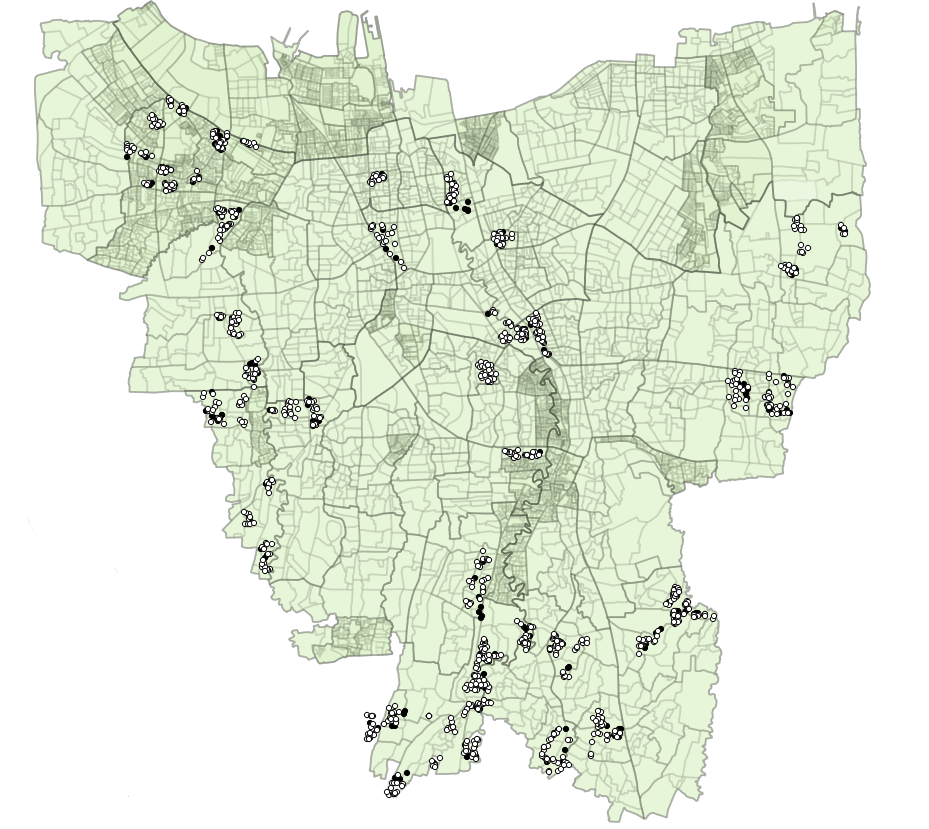
\includegraphics[width=120mm]{FigmapTC.png}
\end{figure}


\begin{figure}[h!]
    \centering
    \caption{Treatment Distribution across Retailers: Village Pegangsaan}
   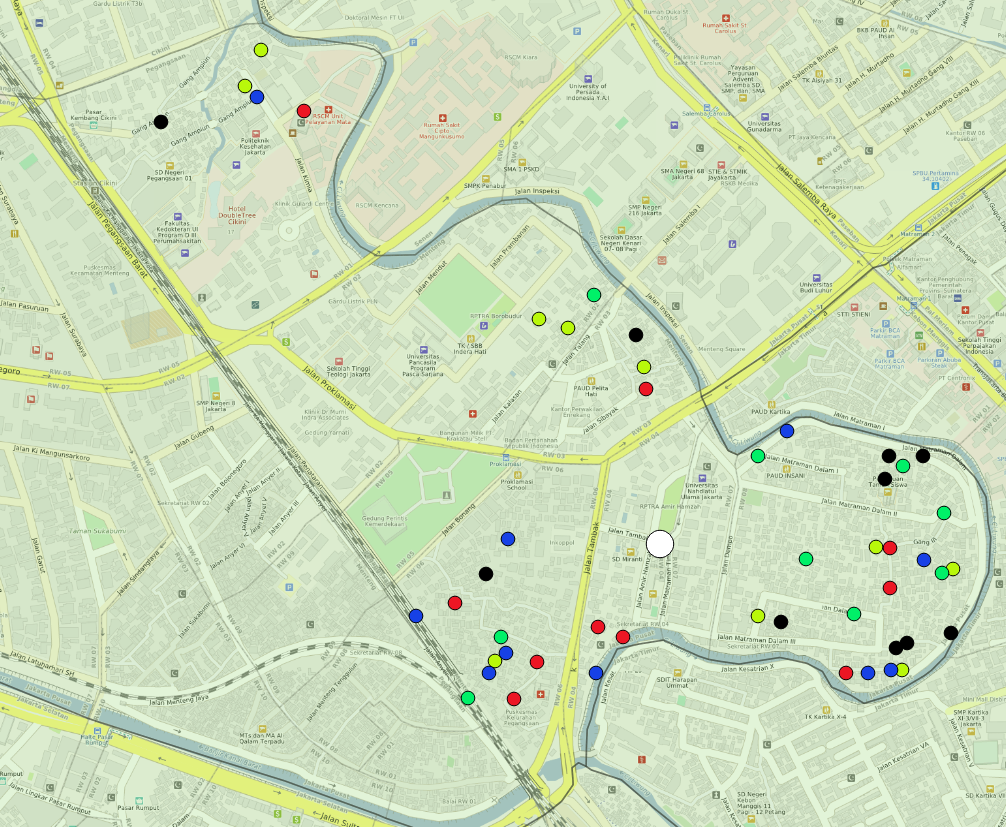
\includegraphics[width=120mm]{FigmapZoom.png}
\end{figure}


\pagebreak

\begin{figure}[h!]
    \centering
    \caption{Movie Screening Locations (big white) and Firms invited to the movie}
   	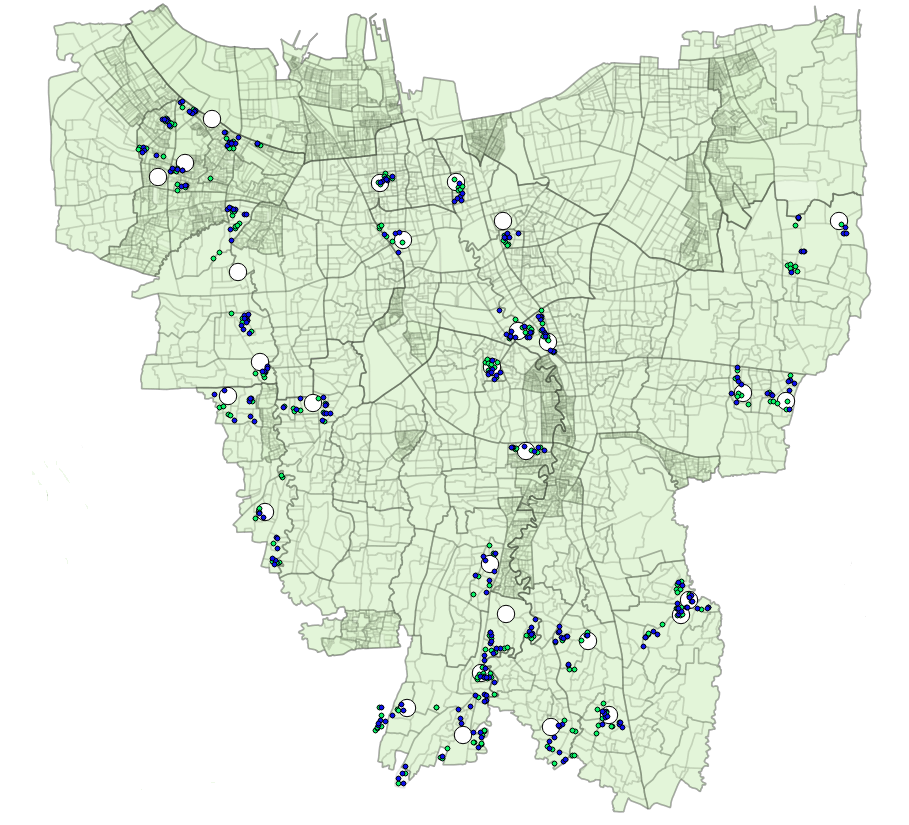
\includegraphics[width=120mm]{FigmapMovie.png}
\end{figure}

\end{landscape}
\pagebreak


\section{Sampling Protocol} \label{sec:appendixd}
\begin{enumerate}

	\item In the order given by the randomized list of selected villages, move 					into a village by approaching the respective head of the village.

	\item Obtain a list of all communities within the respective village and their 				boundaries.
	
	\item Generate a second list that contains these communities in random order.

	\item Move into a village according to the randomized list and, within each 				village, approach the owner of every shop that satisfies the following 				criteria:

	\begin{enumerate}
	
		\item The shop is at a distance of at least 30 meters to any other shop 					already listed.

		\item The shop is not a mere handcart or not otherwise easily moved.

		\item The shop is at least 4 $m^2$ in size

		\item The shop offers products from at least 2 product categories out of 					the following list:

		\begin{enumerate}


			\item Perishables (vegetables, fruits, eggs, rice, etc.)
			\item Pre-packaged food
			\item Soft-drinks and packaged drinks
			\item Snacks
			\item Tobacco
			\item Medicine
			\item Cleaning products
			\item Personal care
			\item DIY products

		\end{enumerate}

		\item The shop owner professes an aspiration to grow their business.

	\end{enumerate}

	\item Conditional upon the shop owner consenting, conduct the interview.

	\item Within the respective community, continue interviewing the owners of all 				shops that satisfy above mentioned criteria.

	\item If at any time the number of shops interviewed within the respective 					village equals or exceeds 67, continue interviewing all shops within 				the communities already moved into, but do not begin sampling in any 				new community within that village.

	\item If and when the total number of shops interviewed equals or exceeds 					2000, continue interviewing all shops within the village until the 					number of shops interviewed within the respective village equals or 				exceeds 67, in which case you continue interviewing all shops within 				the communities already moved into, but do not move into any new 					community within that village (just as outlined above).

\end{enumerate}
\pagebreak
\section{Project Timeline} \label{sec.timeline}

\begin{figure}[h]
    \centering
    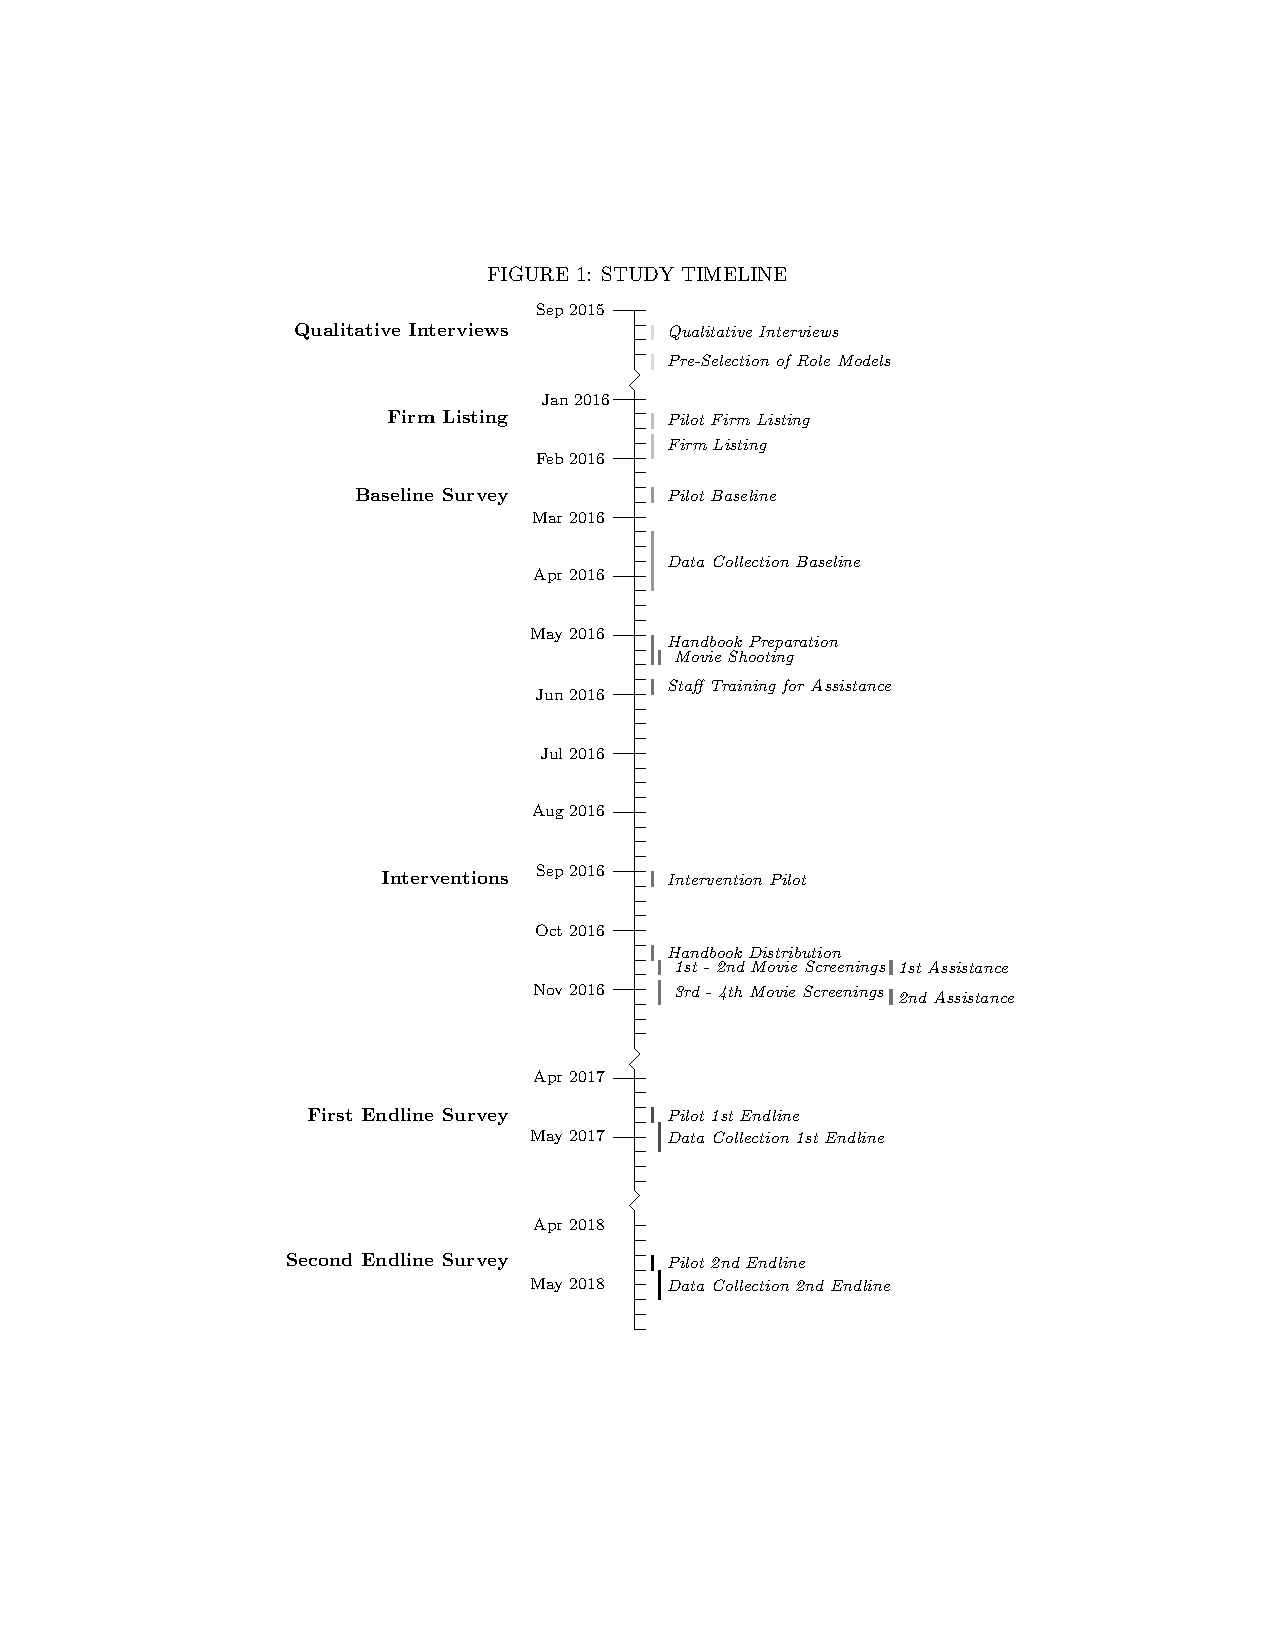
\includepdf[pages=-]{FigTimeline.pdf}
\end{figure}

\pagebreak
\section{Experimental Design} \label{sec:design}

\begin{table}[h!]
  \centering
  \renewcommand{\arraystretch}{1.4}
  \begin{tabular}{|c|c|c|c|c|c|c|c|c|}
    \hline
    \multicolumn{9}{|c|}{\textbf{Total Sample}}\\
    \multicolumn{9}{|c|}{1301 firms}\\
    \hline
    \multicolumn{1}{|c}{\textbf{Control}} & \multicolumn{8}{|c|}{\textbf{Handbooks}}\\
    \multicolumn{1}{|c}{261 firms} & \multicolumn{8}{|c|}{1040 firms}\\
    \cline{2-9}
    \multicolumn{1}{|c}{} & \multicolumn{8}{|c|}{\textbf{Returns to Adoption Framing}}\\
    \cline{2-9}
    \multicolumn{1}{|c}{} & \multicolumn{4}{|c}{\textit{Positive}} & \multicolumn{4}{|c|}{\textit{Negative}}\\
    \multicolumn{1}{|c}{} & \multicolumn{4}{|c}{520 firms} & \multicolumn{4}{|c|}{520 firms}\\
    \cline{2-9}
    \multicolumn{1}{|c}{} & \multicolumn{8}{|c|}{\textbf{Role-Model Movie}}\\
    \cline{2-9}
    \multicolumn{1}{|c}{} & \multicolumn{2}{|c}{\textit{Yes}} & \multicolumn{2}{|c}{\textit{No}} & \multicolumn{2}{|c}{\textit{Yes}} & \multicolumn{2}{|c|}{\textit{No}}\\
    \multicolumn{1}{|c}{} & \multicolumn{2}{|c}{260 firms} & \multicolumn{2}{|c}{260 firms} & \multicolumn{2}{|c}{260 firms} & \multicolumn{2}{|c|}{260 firms}\\
    \cline{2-9}
    \multicolumn{1}{|c}{} & \multicolumn{8}{|c|}{\textbf{Implementation Assistance}}\\
    \cline{2-9}
    \multicolumn{1}{|c}{} & \multicolumn{1}{|c}{\textit{Yes}} & \multicolumn{1}{|c}{\textit{No}} & \multicolumn{1}{|c}{\textit{Yes}} & \multicolumn{1}{|c}{\textit{No}} & \multicolumn{1}{|c}{\textit{Yes}} & \multicolumn{1}{|c}{\textit{No}} & \multicolumn{1}{|c}{\textit{Yes}} & \multicolumn{1}{|c|}{\textit{No}}\\
	\multicolumn{1}{|c}{} & \multicolumn{1}{|c}{130} & \multicolumn{1}{|c}{130} & \multicolumn{1}{|c}{130} & \multicolumn{1}{|c}{130} & \multicolumn{1}{|c}{130} & \multicolumn{1}{|c}{130} & \multicolumn{1}{|c}{130} & \multicolumn{1}{|c|}{130}\\
	\multicolumn{1}{|c}{} & \multicolumn{1}{|c}{firms} & \multicolumn{1}{|c}{firms} & \multicolumn{1}{|c}{firms} & \multicolumn{1}{|c}{firms} & \multicolumn{1}{|c}{firms} & \multicolumn{1}{|c}{firms} & \multicolumn{1}{|c}{firms} & \multicolumn{1}{|c|}{firms}\\
	\hline
  \end{tabular}
\end{table}



\pagebreak
%\section{Selection of Role Models}\label{sec:rolemodel}

%\pagebreak
%\section{Movie Script}\label{sec:movie}

%Available upon request.


\section{Businesses Pictures}\label{sec:expbusinesses}

\begin{figure}[h!]
\centering
\caption{Pictures of two shops representative of the sample of small-scale retail businesses in this study}
\label{warung1}
    \includegraphics[width=120mm]{Warung1.jpg}
\end{figure}

\begin{figure}[h!]
\centering
\label{warung2}
    \includegraphics[width=120mm]{Warung2.png}
\end{figure}

\end{appendices}
\end{document} 